\chapter{Systemmodelle}
\section{Anwendungsfälle}
\subsection{Bedienung der Android App}
\begin{center}
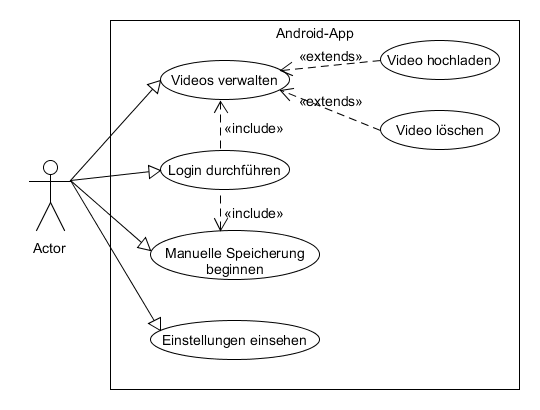
\includegraphics[width=1\textwidth]{subtopicsFuncspec/Res/systemModels/App-AFD-UML.png}
\end{center}
Dieser Anwendungsfall beschreibt die Bedienung der \gls{App}. 
Der Benutzer kann hierbei mehrere Aktionen ausführen:
\begin{itemize}
\itemsep0pt
\item Login durchführen
\item Videos verwalten
\item Manuelle Speicherung beginnen
\end{itemize}
Um die \gls{App} zu nutzen, muss sich der Benutzer zunächst auf der \gls{App} einloggen. Nach dem Einloggen kann der Benutzer sein aufgenommenes Videomaterial verwalten. Er kann z.B. Videos löschen, oder auf den \gls{Web-Dienst} hochladen.
Ist er in der Beobachtungsansicht, so ist es dem Nutzer möglich die Manuelle Speicherung des Videomaterials zu iniziieren.

\subsection{Bedienung der Website}
\begin{center}
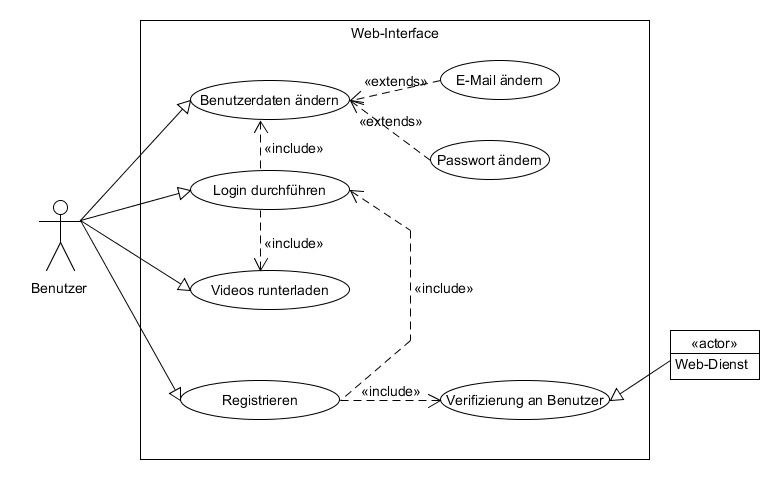
\includegraphics[width=1\textwidth]{subtopicsFuncspec/Res/systemModels/WebsiteAWFDiagram.png}
\end{center}	
Dieser Anwendungsfall beschreibt die Bedienung der Website.
Der Benutzer kann hierbei mehrere Aktionen ausführen:
\begin{itemize}
\itemsep0pt
\item Login durchführen
\item Registrieren
\item Benutzerdaten ändern
\item Verifizierung an Benutzer
\end{itemize}
Um die Website zu nutzen, muss sich der Benutzer zunächst registrieren. Nach der Registrierung und Änderung von Benutzerdaten schickt der \gls{Web-Dienst} eine Verifizierungs-\gls{E-Mail} an den Benutzer. Nach der Bestätigung kann sich er sich auf der Webseite anmelden um deren Funktion zu nutzen. Ist der Benutzer eingeloggt, kann er seine Benutzerdaten ändern und zuvor hochgeladene, nun anonymisierte Videodaten herunterladen.

\section{Aktivitätsdiagramm}
\subsection{Von Appstart bis Videofreigabe}
\begin{center}
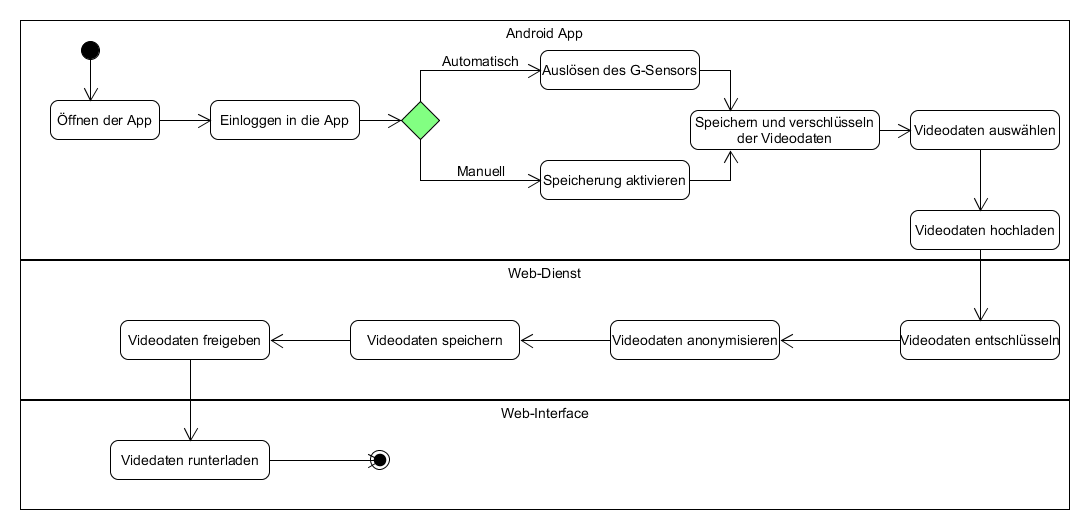
\includegraphics[width=1\textwidth]{subtopicsFuncspec/Res/systemModels/AKDiagramm.png}
\end{center}
Dieses Aktivitätsdiagramm beschreibt den Ablauf vom Start der \gls{App} bis zur Freigabe und dem Runterladen der Videodaten. 
\begin{enumerate}
\itemsep0pt
\item Öffnen der \gls{App}
\item Einloggen in die \gls{App}
\begin{description}
\item Der Benutzer loggt sich mit seinen Anmeldedaten in die \gls{App} ein um die Funktionen zu nutzen.
\end{description}
\item Speicherung beginnen
\begin{enumerate}
\item Auslösen des \gls{G-Sensor}
\begin{description}
\item Der \gls{G-Sensor} löst aus da er den festgelegten Richtwert überschritten hat.
\end{description}
\item Manuelle Speicherung aktivieren
\begin{description}
\item Der Benutzer fordert manuell die Speicherung an.
\end{description}
\end{enumerate}
\item Speichern und verschlüsseln der Videodaten
\begin{description}
\item Nach Beendigung der Aufnahme werden die Videodaten verschlüsselt und daraufhin auf dem Smartphone gespeichert.
\end{description}
\item Videodaten auswählen
\item Videodaten hochladen
\begin{description}
\item Die ausgewählten Videodaten wird auf den \gls{Web-Dienst} hochgeladen.
\end{description}
\item Videodaten entschlüsseln
\item Videodaten \gls{anonymisieren}
\begin{description}
\item Nach der Entschlüsselung der Videodaten, anonymisiert der \gls{Web-Dienst} diese.
\end{description}
\item Videodaten speichern
\item Videodaten freigeben
\begin{description}
\item Die Videodaten werden dem Benutzer auf der \gls{Web-Interface} zugänglich gemacht.
\end{description}
\item Videodaten herunterladen
\begin{description}
\item Nun kann der Benutzer sich einloggen und die anonymisierten Videodaten herunterladen.
\end{description}
\end{enumerate}